\subsection{Desarrollo de la idea}

A partir de un grafo original de $ n $ nodos, representado por un arreglo de nodos de longitud $ n $, donde cada nodo se representa con una clase $ Nodo $ que contiene los atributos $ id $ de tipo \textbf{int}, que indica el índice de cada nodo en el arreglo,  $  color $ de tipo \textbf{int} con el color con que se pinta el grafo, $ tieneColor $ de tipo \textbf{bool}, que indica si se pinto alguna vez el nodo, $ sucesores $ de tipo \textbf{List$ < $Nodo$ > $}, que indica cuales son los sucesores de ese nodo en el grafo, $ coloresPosibles $ de tipo \textbf{List$<$Nodo$>$}, que indica cuales son los posibles colores para el nodo. En el ejercicio dos, se irán sacando colores de esta lista, una vez que los mismos son descartados en el backtracking. Por ultimo el atributo $ coloresOriginales $, se tipo \textbf{Set$<$Nodo$>$} que sera utilizado en el ejercicio dos para reponer los colores originales. A partir de este grafo construimos uno de proposiciones, también representado por un arreglo de nodos, pero para estos utilizamos la clase $ NodoP $. El arreglo tiene tamaño $ 4 n $, ya que por cada nodo tenemos cuatro nodos de proposiciones. Si tiene dos colores, tenemos por cada uno la afirmación y negación de que tiene cierto color. Si el nodo tiene un solo color, tenemos solo la afirmación.

 La forma de dirigirse en los índices del grafo de proposiciones , es primero aparecen las afirmaciones, y después las negaciones respectivamente, por cada nodo original tenemos cuatro de proposiciones en ese orden. Para el caso de un nodo con un solo color, igualmente se ocupan cuatro posiciones en el arreglo, pero los nodos de las mismas se setean como vacíos. La clase $ NodoP $, tiene los atributos: \textbf{int id}, indica el índice en el arreglo, \textbf{int nNodoAsociado}, que indica sobre que número de nodo habla la proposición, \textbf{int colorAsociado}, que indica sobre que color habla la proposición, \textbf{boolean esNegacion}, que nos dice si la propocición se corresponde con una negación o con una afirmación, \textbf{List$<$NodoP$>$ sucesores}, que nos dice cuales son los sucesores, \textbf{int valorDeVerdad}, que nos da el valor de verdad que determinamos para la proposición, el mismo puede ser 0 si es falsa, 1 si es verdadera, 2 si todabía no se determino el valor de verdad, \textbf{boolean marcado} que sirve para ir marcando los nodos en la búsqueda bfs, \textbf{boolean esVacio}, que sirve en caso de tener nodos con un solo color.
 
Implementamos la función $ noSePuedePintar $, que toma como entrada un grafo, y nos devuelve verdadero en caso de que no se pueda pintar, y en caso contrario falso, y además pinta el grafo. Para esto, a partir del grafo original, construimos un grafo donde una proposición tiene como sucesora a otra, si esta ultima es implicada por la primera. De esta manera, para las cuatro proposiciones asociadas a un nodo, como este ultimo solo puede tener un color, tenemos que en caso de haber dos colores posibles, la afirmación de un color implica la negación del otro, y viceversa. Luego de establecer estas relaciones en el grafo de proposiciones, utilizamos la información del grafo original para continuar estableciendo relaciones, la afirmación de un color en un nodo implica la negación de ese color en los nodos adyacentes, en caso de que el mismo lo posea. Hay que destacar que en el grafo de proposiciones, que por la transitividad de la implicación una proposición implica otra si y solo si, existe un camino en el grafo desde la hipótesis a la tesis.

Una vez construido el grafo de proposiciones, aplicamos el algoritmo de Kosaraju, explicado en el laboratorio, para obtener las componentes fuertemente conexas, es decir los conjuntos de nodos tales que dados dos de ellos hay un camino de uno hacia el otro y viceversa. Implementamos la función $ componentesFuertementeConexas $ que nos devuelve una lista con las componentes fuertemente conexas. Las proposiciones en la misma componente son todas equivalentes, por lo que deben tener el mismo valor de verdad. En caso de que una afirmación y su negación se encuentren en la misma componente conexa, no podrá ser posible pintar el grafo, por lo que se devolverá falso. 

En caso de que no halla contradicciones, utilizamos bfs para saber si hay un camino desde una negación($ \neg C $) de una proposición a su respectiva afirmación ($ C $). En este caso, como la implicación debe ser verdadera, la hipótesis debe ser falsa, es decir $ C $ debe ser falsa. De la misma manera nos fijamos si hay un camino desde una afirmación($ C $) a una negación ($ \neg C $). En este caso, como la hipótesis debe ser falsa, la afirmación también. Además seteamos en falso los elementos de la componente conexa a la que pertenece esa proposición, ya que todos los elementos de una misma componente conexa debe tener el mismo valor de verdad. 

El valor de verdad de una proposición, como cada nodo puede pintarse de un solo color, determina el valor de verdad de las cuatro proposiciones asociadas a un nodo. Entonces lo siguiente que hacemos es a partir de los valores de verdad obtenidos anteriormente, complementar las proposiciones asociadas a ese nodo.

Luego como para que una implicación sea verdadera, es necesario que en caso de que la hipótesis sea verdadera, la tesis también, procedemos a propagar el valor de verdad de las proposiciones verdaderas a sus implicaciones, para esto utilizamos la función $ cambiarSucesores $. Luego, tal como puede verse en el pseudocódigo , volvemos a completar los cuatro colores. Finalmente, en caso de quedar proposiciones con valor de verdad dos, le asignamos algún valor de verdad, teniendo cuidado de en cada paso propagar los verdaderos, y completar los cuatro colores.

Una vez que tenemos todos los valores de verdad para el grafo de proposiciones, procedemos a pintar el grafo original, pintando los nodos de afirmaciones con valor de verdad verdadero.

\subsection{Complejidad y pseudocódigo}
En el siguiente fragmento podemos encontrar el pseudocódigo y de complejidad del algoritmo, para detalles del calculo de complejidad, ver apéndice.

\begin{codebox}
\Procname{$\proc{noSePuedePintar}( Nodo[]\ nodosGrafo) $ $\longrightarrow res:Bool$}
	\li  Crear el grafo de proposiciones en base al original// $O(4n*min(n,m))$
	\li Calcular las componentes fuertemente conexas del grafo de proposiciones con el algoritmo de kosaraju. \li \Comment{Costo kosaraju} $ O( n +m ) $
	\li Revisar las componentes para ver si hay alguna proposición y su respectiva negación en una misma 
	\li componente, costo en peor caso menor o igual a $ O(n^{2}) $.
	\li En caso de encontrar, finalizar y retornar verdadero, lo cual quiere decir que no se puede pintar.
	\li \For $\  NodoP \ nopd $ \To $ grafoProposiciones$ \Do	
	\li			\If $ esNegacion(nopd)$
	\li	\Then $aplicar \ bfs\ para\ saber\ si\ hay\ un\ camino\ desde\ la\ negacion\ a\ su\ respectiva\ afirmacion$
	\li \Comment{En este caso setear la afirmación en verdadera. Costo $O( n + m )$ }						

				\End
	\li		\Then		\Else $ aplicar\ bfs\ para\ saber\ si\ hay\ un\ camino\ desde\ la\ afirmacion a\ su\ respectiva\ negacion$
\li \Comment{En este caso setear la afirmacion en falsa, y todas las de su componente conexa en  falso. Costo$O( n + m )$ }						
			\End
\li	\textbf{end if}\End
\End
	\li \textbf{end for}\Comment{Costo ciclo $ O(4n(n+m)) $ }	
	\li Sabiendo el valor de un nodo de proposición asociado a un nodo del grafo original, calculamos el valor \li de verdad de los cuatro restantes. Costo $ O(n) $
	\li Expandimos los verdaderos en el grafo de proposiciones, es decir seteamos en verdadero todas las \li implicaciones de un verdadero. Costo $ O(n^2) $
	\li Volvemos a completar el valor de verdad cada cuatro proposiciones. $ O(n) $
	\li \For $\  NodoP \ nopd $ \To $ grafoProposiciones$ \Do	
	\li	\Then		\If $ nodp\ tiene\ valor\ de\ verdad\ de\ dos$
	\li	\Then $completar\ asignarle\ un\ valor\ de\ verdad\ al\ mismo,\ y\ a\ las\ cuatro\ asociadas$
	\li $Expandir el valor de verdad de las proposiciones seteadas como verdaderas.$ $ O(n) $
	\li $Completar el valor de verdad de los cuatro nodos asociados.$ $ O(n) $
		\End
	\li \textbf{end if}	$ O(n^2) $	\End
	\li \textbf{end for}
	\li Recorrer el grafo de proposiciones, y pintar los nodos del grafo original con los colores dados por \li las afirmaciones verdaderas. Costo $ O(n) $
				      
\end{codebox}

Tenemos un costo total de $ O(n^2 + n*m) $. Complejidad del algoritmo de kosaraju para obtener las componentes fuertemente conexas:

\begin{codebox}
\Procname{$\proc{componentesFuertementeConexas}( Nodo[]\ nodosGrafo) $ $\longrightarrow res:List<Stack<NodoP>>$}
	\li  Crearmos una pila nueva, y aplicamos un dfs recursivo, que apila en la misma los nodos 
	\li que va visitando, en el orden inverso al que fueron visitados, es decir primero apila los últimos
	\li visitados, por lo que estos quedaran en el fondo de la pila. Costo $ O(n+ mp) $, o $ O(n + m) $
	\li Obtener el grafo inverso. Costo $ O(mp) $ o $ O(n + m) $
	\li En caso de encontrar, finalizar y retornar verdadero, lo cual quiere decir que no se puede pintar.
	\li List$<$Stack$<$NodoP$>>$ componentes = new ArrayList$<>$();  	\Comment{Donde almacenaremos las componentes }
	\li \While $ esNoVacia(orden)$ \Do	
	\li NodoP nn= orden.pop()
	\li			\If $ noEstaMarcado(nn)$
	\li	\Then $Crear \ nueva\ pila \ donde \se \ almacenara \ una\ nueva \ componente$
	\li $ Aplicar\ dfs \ recursivo\ teniendo\ en\ cuenta\ los\ nodos\ marcados\ globalmente, \ apilando\ al$ \li $igual\ que\ antes\ los\ nodos\ en \ la \ nueva\ pila $
	\li $ Agregar\ la\ componente\ a\ la\ lista\ de\ componentes $
	 		\End						
	\li \textbf{end if}		\End
\li \textbf{end while} \Comment{Costo $ O(n+mp) $ o $ O(n + m) $}		
	\li Retornar la lista de componentes

\end{codebox}

Tenemos un costo de $ O(n + m) $ para kosaraju.


\subsection{Experimentación}

Se analizaran solo grafos generados aleatoriamente. Teniendo en cuenta las tres variables ($ c $, $ n $, y $ m $), se llevaron a cabo tres experiencias, en cada una se dejan fijas dos de las variables, y se varia la restante. Como el tiempo de computo era bien distinto para los casos en que no se podía pintar el grafo, del que si se podía, ya que este ultimo involucra todo el proceso de pintado, se clasificaron los resultados según este criterio.

Para generar instancias se utilizaron generadores de instancias en java, y par tomar tiempos se utilizo la clase de java $ Ej2Tiempos $, en la cual para cada instancia se corre 30 veces el algoritmo, se guardan los resultados en un arreglo. Calculamos el promedio  y el desvío estándar del mismo, y luego lo filtramos quedándonos con los valores que estuvieran entre el promedio menos el desvío estándar y promedio mas el desvío estándar. Finalmente tomamos un promedio de los valores que quedaron, y ese es el resultado que consideramos como tiempo final.

 En los siguientes gráficos podemos visualizar los resultados.

\begin{figure}[H]
 \begin{center}
     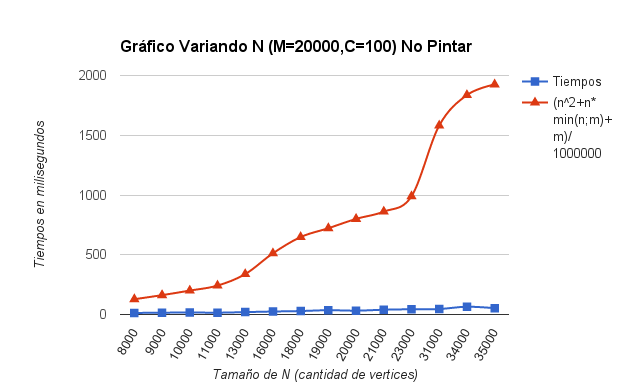
\includegraphics[scale=0.6]{../Ejercicio1VariandoNNoPintar.png}
 \end{center}
 \caption{Tiempos ejercicio 1, variando N, casos en los que no se puede pintar}
 \label{nnop}
\end{figure}



\begin{figure}[H]
 \begin{center}
     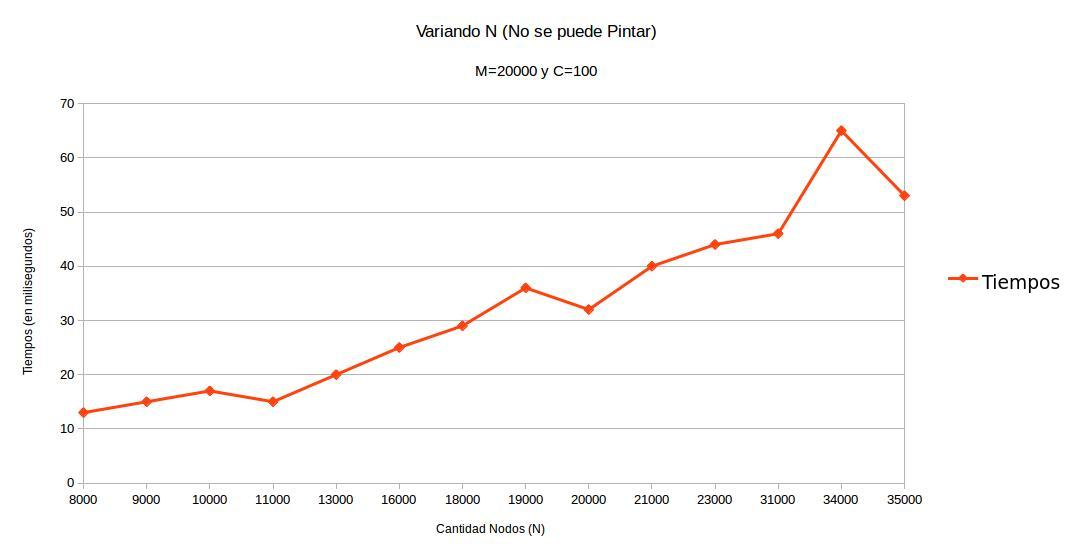
\includegraphics[scale=0.45]{../M20000C100VariandoNnoSePuedePintar.jpg}
 \end{center}
 \caption{Tiempos ejercicio 1, variando N, casos en los que no se puede pintar, visto con zoom}
 \label{nnopz}
\end{figure}

Según las figuras \ref{nnop} y \ref{nnopz},a pesar de que no se pudo pintar el grafo, se puede notar un incremento en el tiempo de computo al incrementar N.

\begin{figure}[H]
 \begin{center}
     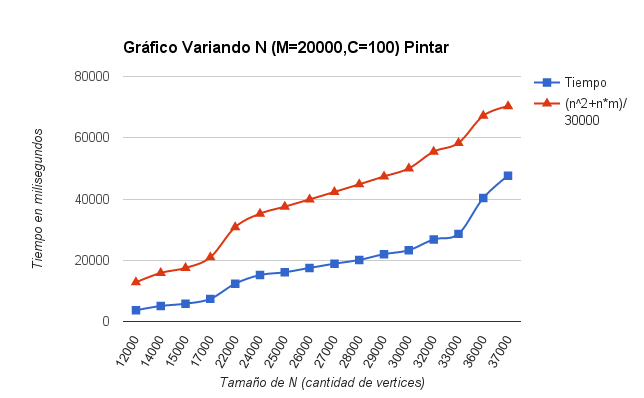
\includegraphics[scale=0.6]{../Ejercicio1VariandoNPintar.png}
 \end{center}
 \caption{Tiempos ejercicio 1, variando N, casos en los que se puede pintar}
 \label{n}
\end{figure}

En la figura \ref{n} se puede notar un claro aumento en el tiempo de computo al incrementar N.


%\begin{figure}[H]
% \begin{center}
%     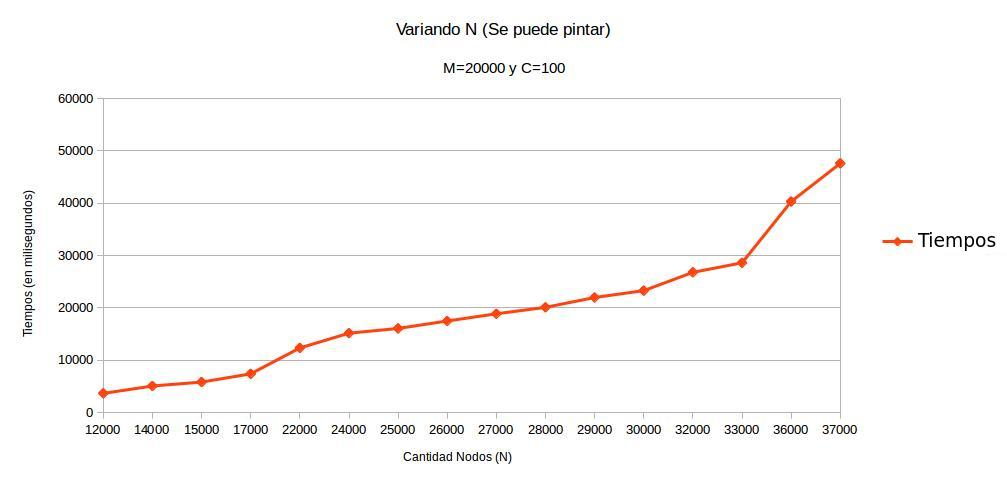
\includegraphics[scale=0.45]{../M20000C100VariandoNSePuedePintar.jpg}
% \end{center}
% \caption{Tiempos ejercicio 1, variando N, casos en los que se puede pintar, visto con zoom}
%\end{figure}



\begin{figure}[H]
 \begin{center}
     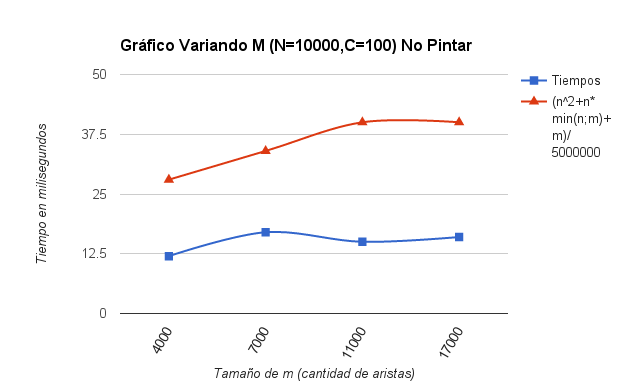
\includegraphics[scale=0.6]{../Ejercicio1VariandoMNoPintar.png}
 \end{center}
 \caption{Tiempos ejercicio 1, variando M, casos en los que no se puede pintar}
\end{figure}



\begin{figure}[H]
 \begin{center}
     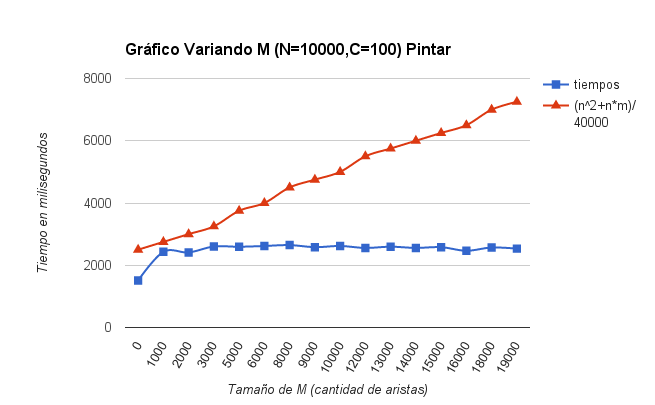
\includegraphics[scale=0.6]{../Ejercicio1VariandoMPintar.png}
 \end{center}
 \label{m}
 \caption{Tiempos ejercicio 1, variando M, casos en los que se puede pintar}
\end{figure}


\begin{figure}[H]
 \begin{center}
     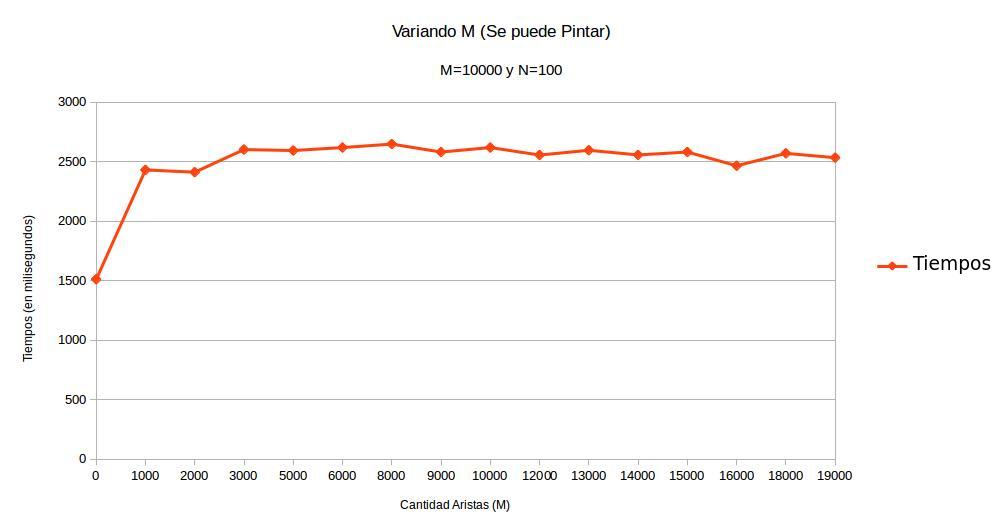
\includegraphics[scale=0.45]{../N10000C100VariandoMSePuedePintar.jpg}
 \end{center}
 \label{mz}
 \caption{Tiempos ejercicio 1 variando M, casos en los que se puede pintar, visto con zoom}
\end{figure}

En base al los gráficos de las figuras~\ref{m} y \ref{mz}, no se noto un incremento en el tiempo de computo, al incrementar M, como podría esperarse, a pesar de que se utilizo un rango amplio. La complejidad obtenida puede considerarse constante.

\begin{figure}[H]
 \begin{center}
     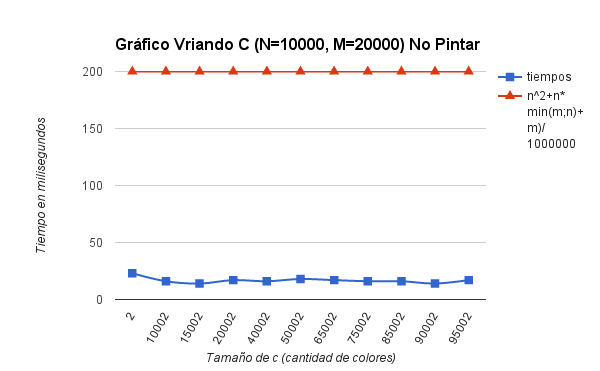
\includegraphics[scale=0.6]{../Ejercicio1VariandoCNoPintar.png}
 \end{center}
 \caption{Tiempos ejercicio 1, variando C, casos en los que no se puede pintar}
 \label{Cno}
\end{figure}

\begin{figure}[H]
 \begin{center}
     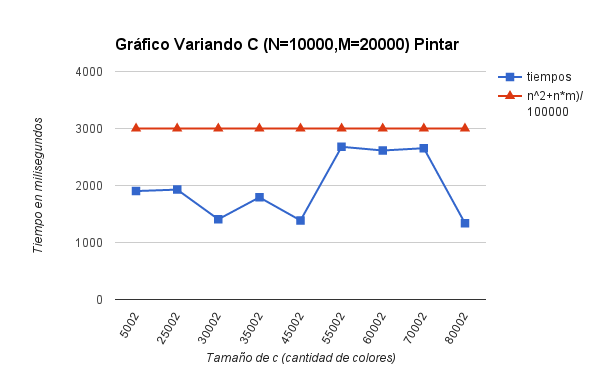
\includegraphics[scale=0.6]{../Ejercicio1VariandoCPintar.png}
 \end{center}
 \caption{Tiempos ejercicio 1, variando C, casos en los que se puede pintar}
 \label{Csi}
\end{figure}

En las figuras \ref{Cno} y \ref{Csi}, se utilizo un rango amplio para los valores de C, pero no se encontró algún crecimiento o decrecimiento considerable en el tiempo de computo. La complejidad obtenida puede considerarse constante.